\section{Suddivisione del lavoro e prospetto economico}
In questa sezione verr\'a trattato come il team \gruppo ha suddiviso i vari ruoli definiti in \NormeDiProgetto~ nei vari periodi, in modo da rispettare il vincolo fornito dal docente riguardo la rotazione dei ruoli.
\subsection{Analisi}
Per quanto riguarda questo periodo, nonostante i costi prodotti in questo lasso di tempo non siano a carico del committente, vengono riportati ugualmente per avere una visione d' insieme dell' operato del gruppo.\\
\subsubsection{Suddivisione dei ruoli}
\begin{center}
\begin{tabular}{| l | c | c | c | c | c | c | c |}
\hline
Membro & Re & Am & An & Pt & Ve & Pr & ore totali \\
\hline
Botter Marco & 0 & 0 & 20 & 0 & 4 & 0 & 24 \\

Giachin Vanni & 0 & 0 & 18 & 0 & 10 & 0 & 28 \\

Marcomin Gabriele & 0 & 0 & 20 & 0 & 4 & 0 & 24 \\

Quaglio Davide & 30 & 0 & 0 & 0 & 0 & 0 & 30 \\

Santangelo Davide & 0 & 14 & 0 & 0 & 8 & 0 & 22 \\

Seresin Davide & 0 & 20 & 6 & 0 & 4 & 0 & 30 \\
\hline
Ore totali & 30 & 34 & 64 & 0 & 30 & 0 & 158 \\
\hline
\end{tabular}
\\
Tabella 3: Ore per membro, periodo di Analisi.
\end{center}
\setlength{\unitlength}{1mm}\begin{picture}(15,60)
                \put(10,0){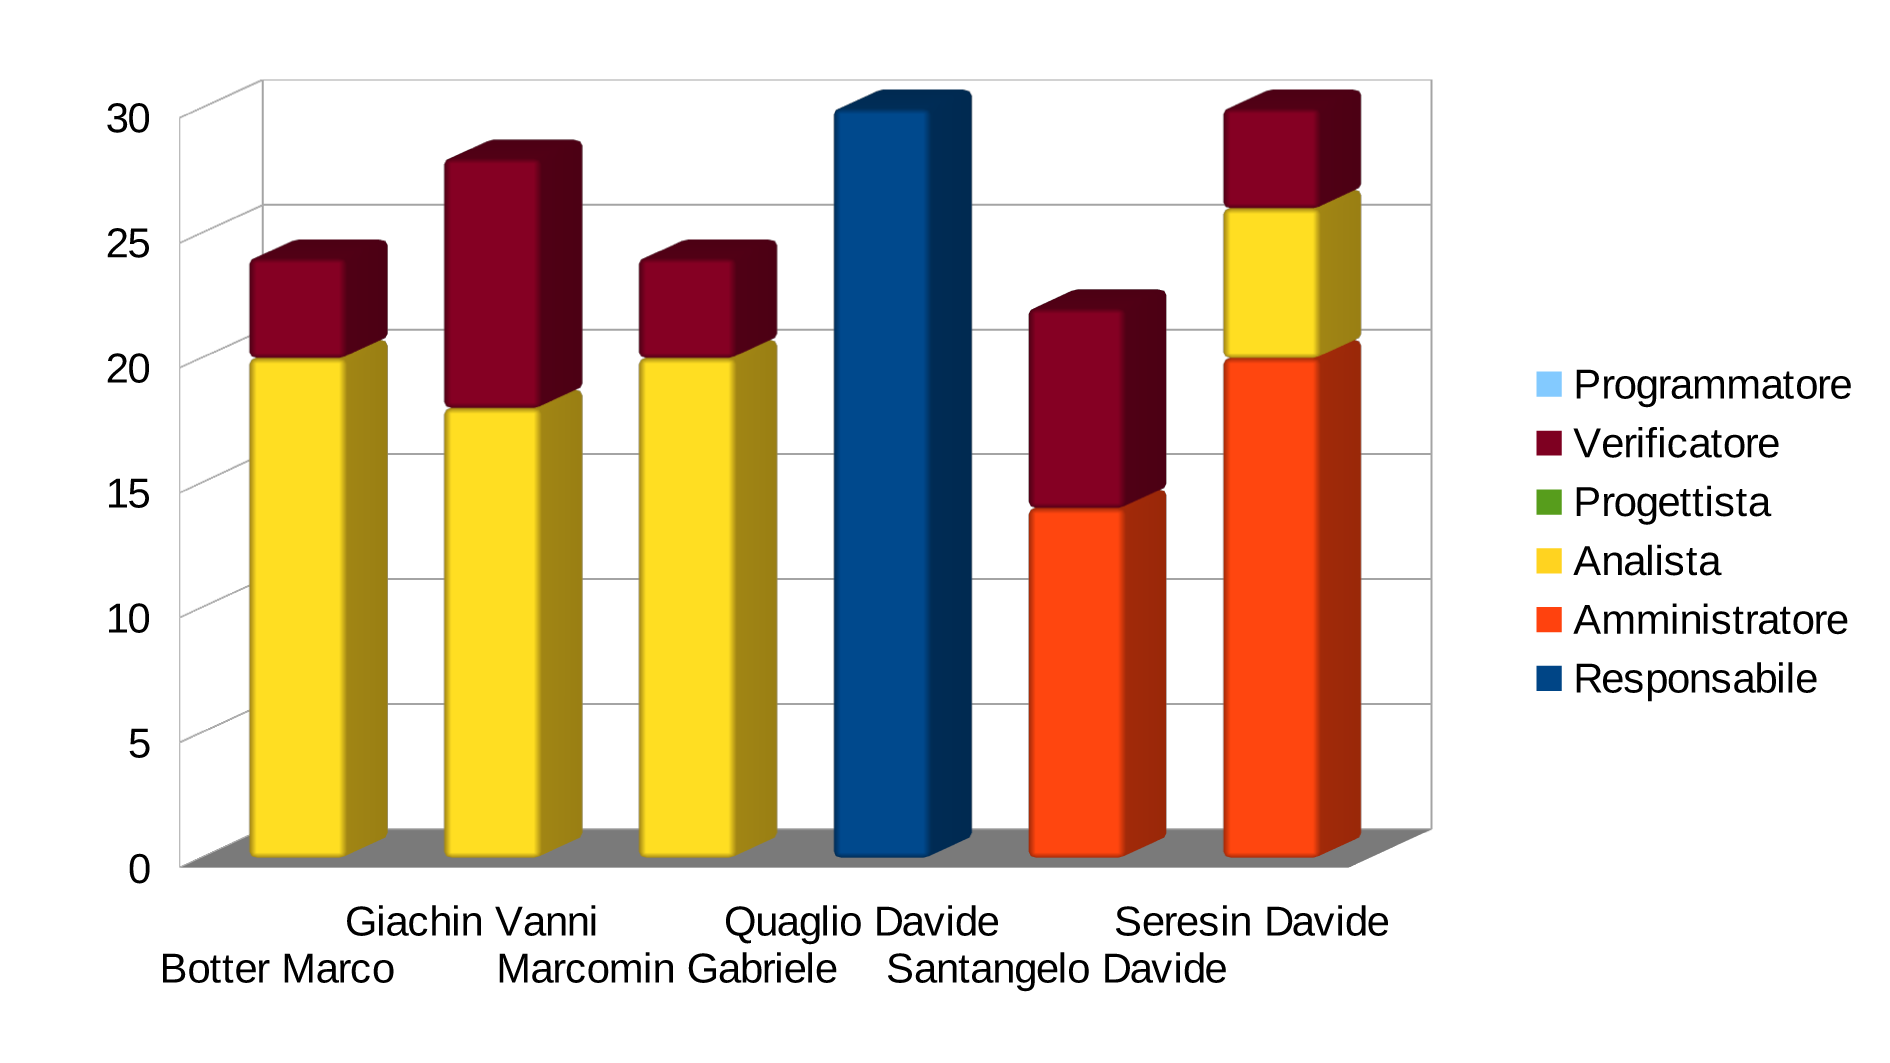
\includegraphics[scale=0.7]{../modello/img/1.png}}
        \end{picture}
\begin{center}
Grafico 1: Ore per componente periodo di Analisi.
\end{center}
\subsubsection{Prospetto economico}
\begin{center}
\begin{tabular}{| l | c | c |}
\hline
Ruolo & Ore & Costi \\
\hline
Responsabile & 30 & 900 \\
Amministratore & 34 & 680 \\
Analista & 64 & 1600 \\
Progettista & 0 & 0 \\
Verificatore & 30 & 450 \\
Programmatore & 0 & 0 \\
\hline
\textbf{Totale} & 158 & 3630 \\
\hline
\end{tabular}
\\
	Tabella 4: Tabella del prospetto economico.
\end{center}
\subsection{Progettazione Architetturale}
\subsubsection{Suddivisione dei ruoli}
\begin{center}
\begin{tabular}{| l | c | c | c | c | c | c | c |}
\hline
Membro & Re & Am & An & Pt & Ve & Pr & ore totali \\
\hline
Botter Marco & 4 & 0 & 0 & 20 & 4 & 0 & 28 \\

Giachin Vanni & 0 & 0 & 6 & 20 & 2 & 0 & 30 \\

Marcomin Gabriele & 0 & 7 & 4 & 15 & 4 & 0 & 30 \\

Quaglio Davide & 2 & 0 & 8 & 20 & 0 & 0 & 30 \\

Santangelo Davide & 0 & 5 & 10 & 0 & 10 & 0 & 25 \\

Seresin Davide & 0 & 0 & 6 & 20 & 2 & 0 & 28 \\
\hline
Ore totali & 6 & 12 & 34 & 95 & 22 & 0 & 169 \\
\hline
\end{tabular}
\\
Tabella 5: Ore per membro, periodo di Analisi
\end{center}
\setlength{\unitlength}{1mm}\begin{picture}(15,60)
                \put(10,0){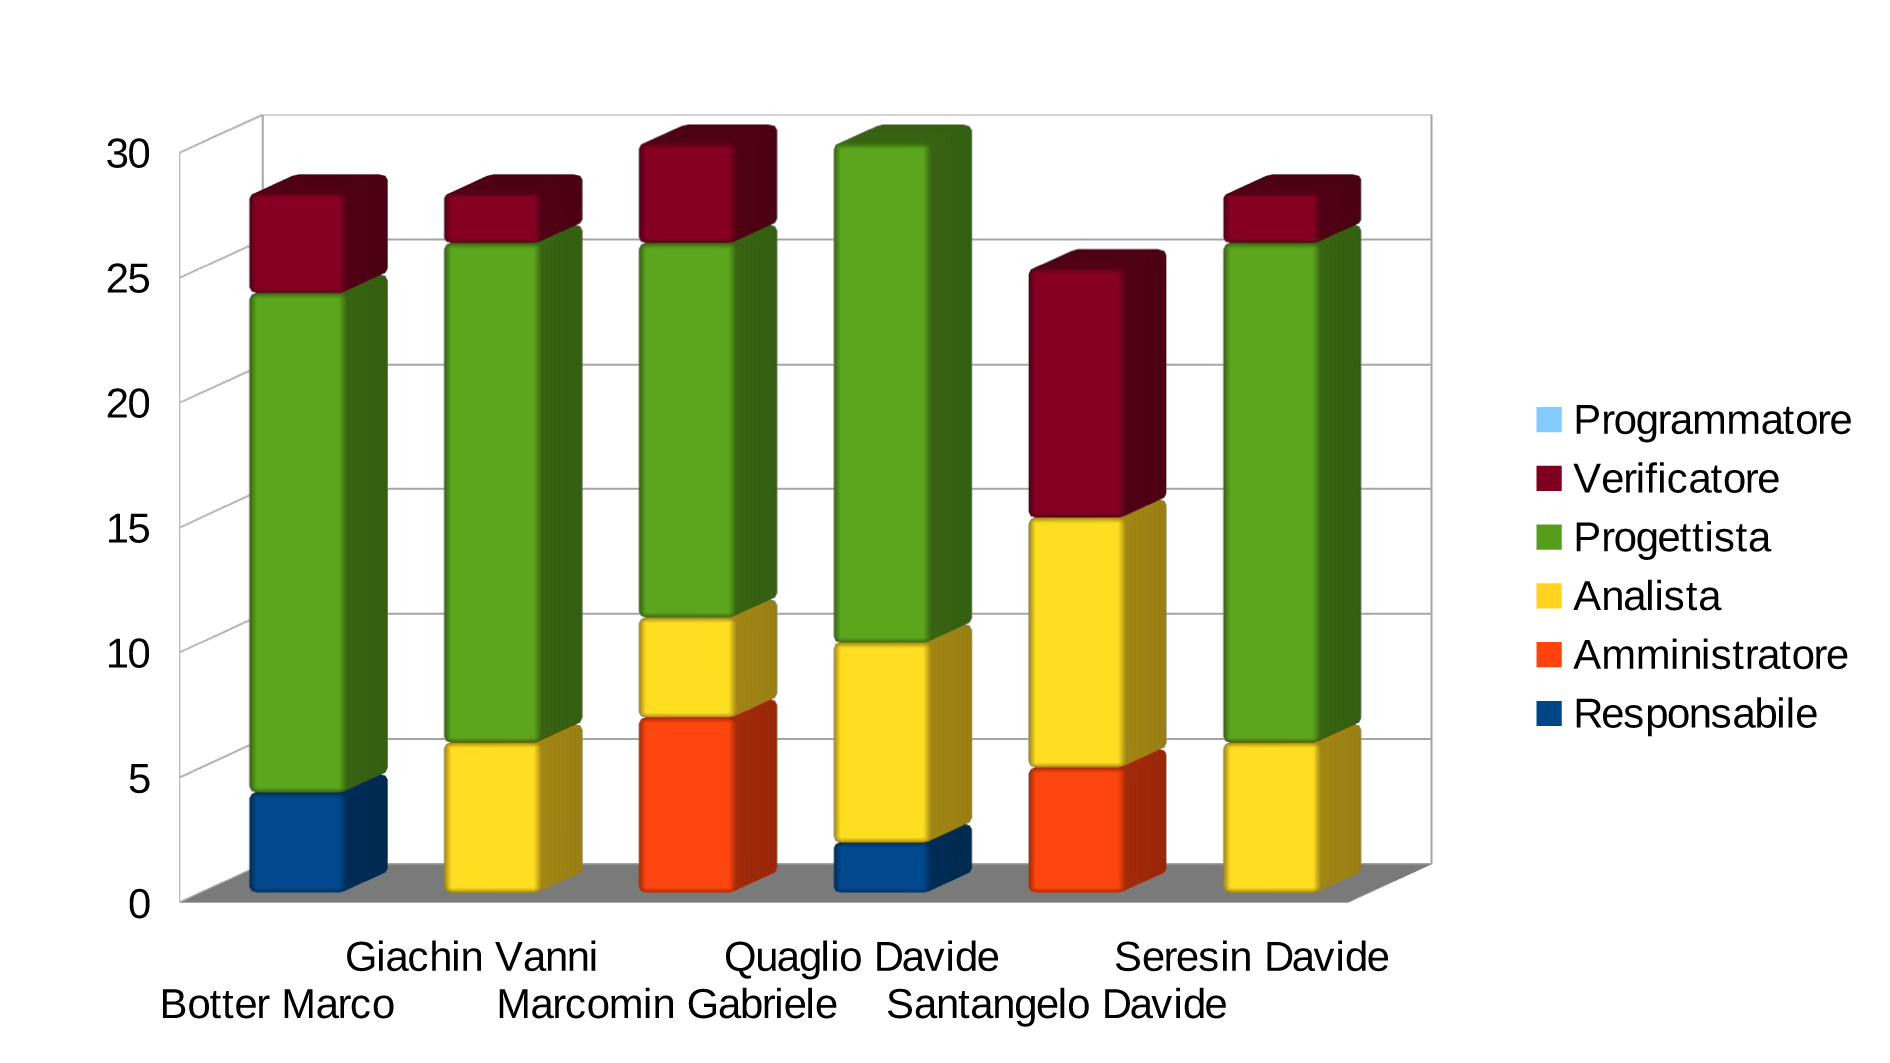
\includegraphics[scale=0.7]{../modello/img/2.png}}
        \end{picture}
\begin{center}
Grafico 2: Ore per componente periodo di Progettazione Architetturale.
\end{center}
\subsubsection{Prospetto economico}
\begin{center}
\begin{tabular}{| l | c | c |}
\hline
Ruolo & Ore & Costi \\
\hline
Responsabile & 8 & 240 \\
Amministratore & 14 & 280 \\
Analista & 44 & 1100 \\
Progettista & 105 & 2310 \\
Verificatore & 22 & 330 \\
Programmatore & 0 & 0 \\
\hline
\textbf{Totale} & 193 & 4260 \\
\hline
\end{tabular}
\\
Tabella 6: Tabella del prospetto economico.
\end{center}
\subsection{Progettazione di Dettaglio e Codifica}
\subsubsection{Suddivisione dei ruoli}
\begin{center}
\begin{tabular}{| l | c | c | c | c | c | c | c |}
\hline
Membro & Re & Am & An & Pt & Ve & Pr & ore totali \\
\hline
Botter Marco & 0 & 0 & 0 & 13 & 16 & 16 & 45 \\

Giachin Vanni & 6 & 0 & 0 & 15 & 14 & 17 & 52 \\

Marcomin Gabriele & 4 & 0 & 0 & 0 & 20 & 22 & 46 \\

Quaglio Davide & 0 & 8 & 2 & 15 & 16 & 19 & 60 \\

Santangelo Davide & 0 & 0 & 0 & 24 & 15 & 15 & 54 \\

Seresin Davide & 0 & 0 & 0 & 19 & 20 & 0 & 39 \\
\hline
Ore totali & 10 & 8 & 2 & 86 & 101 & 89 & 296 \\
\hline
\end{tabular}
\\
Tabella 7: Ore per membro, periodo di Progettazione di dettaglio e codifica
\end{center}
\setlength{\unitlength}{1mm}\begin{picture}(15,60)
                \put(10,0){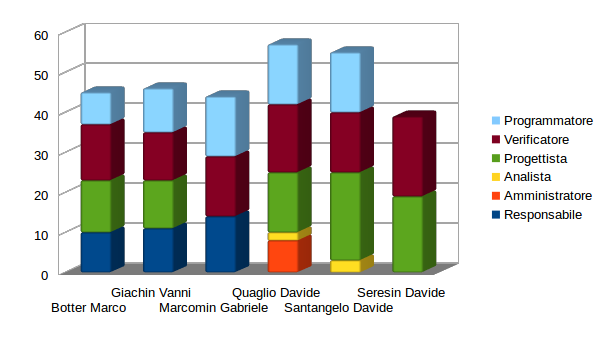
\includegraphics[scale=0.7]{../modello/img/3.png}}
        \end{picture}
\begin{center}
Grafico 3: Ore per componente periodo di Progettazione di Dettaglio e Codifica.
\end{center}
\subsubsection{Prospetto economico}
\begin{center}
\begin{tabular}{| l | c | c |}
\hline
Ruolo & Ore & Costi \\
\hline
Responsabile & 10 & 300 \\
Amministratore & 8 & 160 \\
Analista & 2 & 50 \\
Progettista & 86 & 1892 \\
Verificatore & 101 & 1515 \\
Programmatore & 89 & 1335 \\
\hline
\textbf{Totale} & 296 & 5252 \\
\hline
\end{tabular}
\\
Tabella 8: Tabella del prospetto economico.
\end{center}
\subsection{Verifica e Validazione}
\subsubsection{Suddivisione dei ruoli}
\begin{center}
\begin{tabular}{| l | c | c | c | c | c | c | c |}
\hline
Membro & Re & Am & An & Pt & Ve & Pr & ore totali \\
\hline
Botter Marco & 0 & 10 & 0 & 0 & 17 & 5 & 32 \\

Giachin Vanni & 0 & 10 & 0 & 0 & 15 & 0 & 25 \\

Marcomin Gabriele & 0 & 0 & 0 & 17 & 12 & 0 & 29 \\

Quaglio Davide & 0 & 0 & 0 & 0 & 15 & 0 & 15 \\

Santangelo Davide & 6 & 0 & 0 & 8 & 12 & 0 & 26 \\

Seresin Davide & 5 & 0 & 0 & 5 & 15 & 13 & 38 \\
\hline
Ore totali & 11 & 20 & 0 & 30 & 86 & 18 & 165 \\
\hline
\end{tabular}
\\
Tabella 9: Ore per membro, periodo di Verifica e Validazione.
\end{center}
\setlength{\unitlength}{1mm}\begin{picture}(15,60)
                \put(10,0){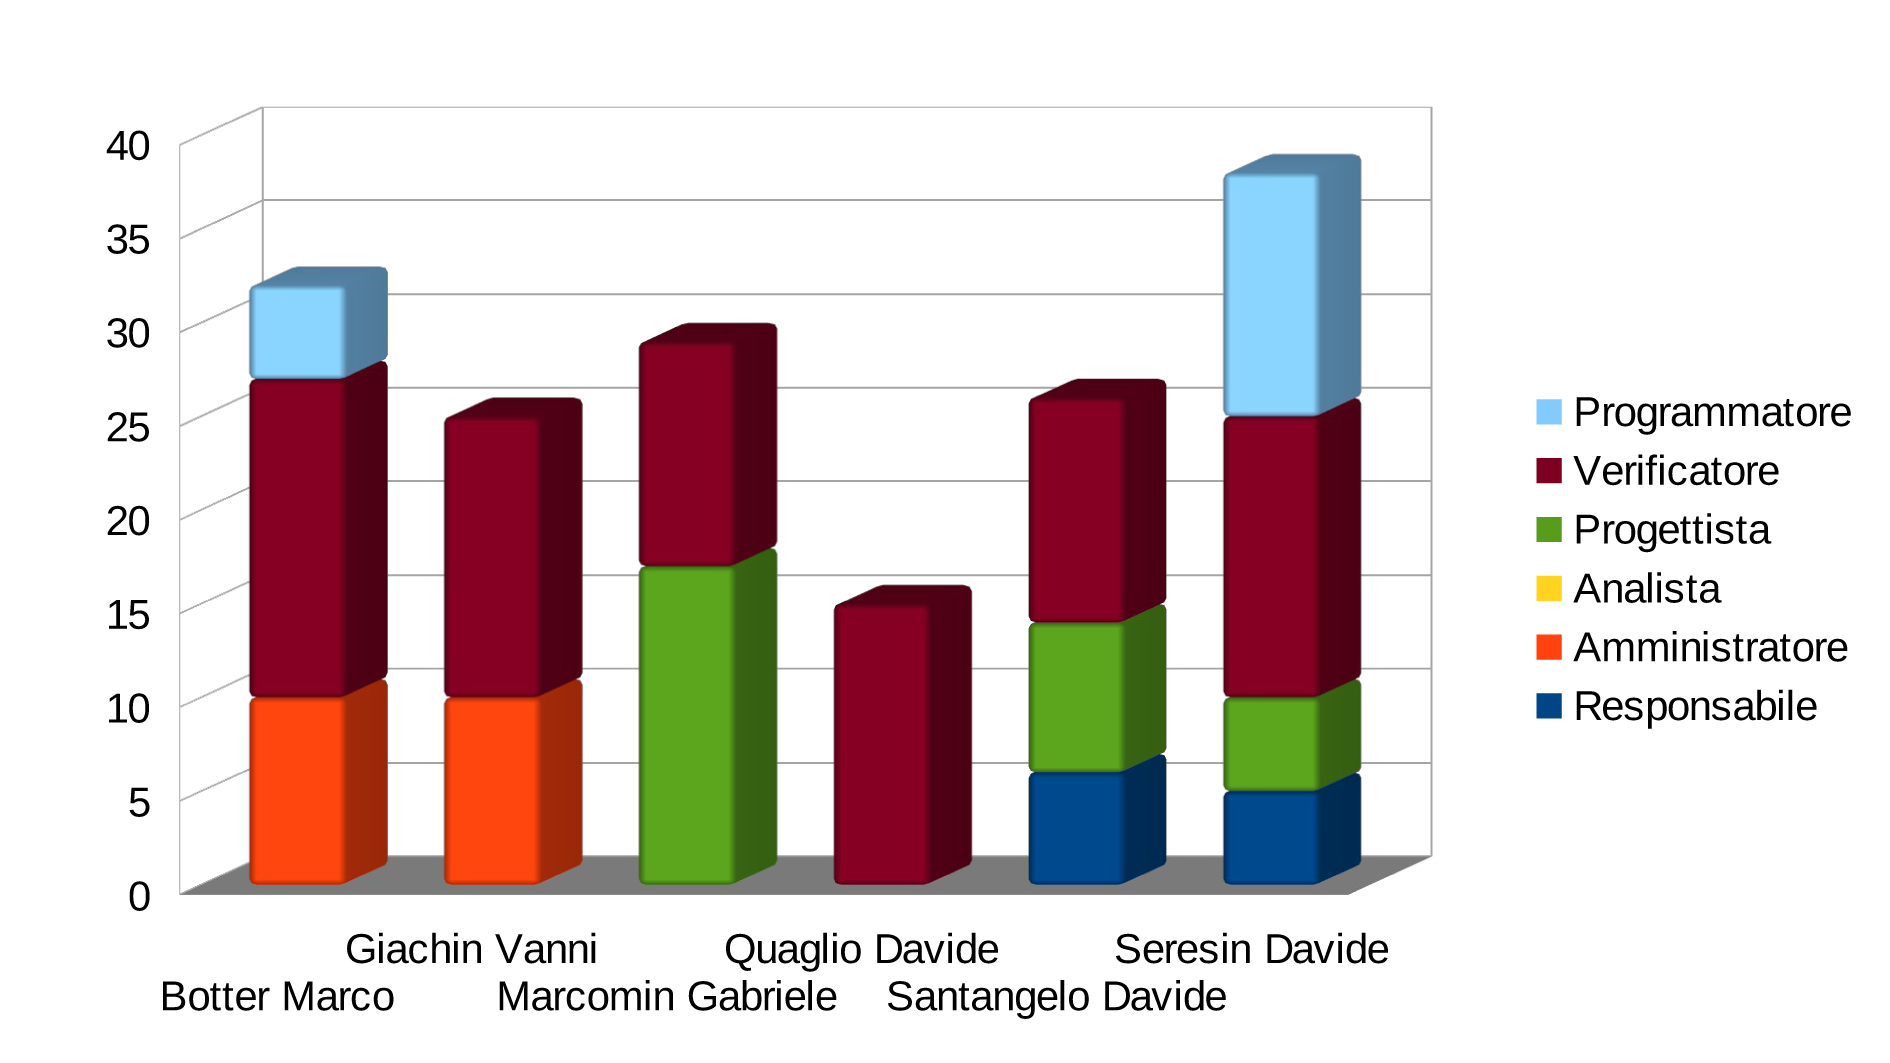
\includegraphics[scale=0.7]{../modello/img/4.png}}
        \end{picture}
\begin{center}
Grafico 4: Grafico ore per componente periodo di Analisi e Verifica.
\end{center}
\subsubsection{Prospetto economico}
\begin{center}
\begin{tabular}{| l | c | c |}
\hline
Ruolo & Ore & Costi \\
\hline
Responsabile & 11 & 330 \\
Amministratore & 20 & 400 \\
Analista & 0 & 0\\
Progettista & 30 & 660 \\
Verificatore & 86 & 1290 \\
Programmatore & 18 & 270 \\
\hline
\textbf{Totale} & 165 & 2950 \\
\hline
\end{tabular}
\\
Tabella 10: Tabella del prospetto economico.
\end{center}
\subsection{Totale}
\subsubsection{Suddivisone dei ruoli con periodo di Analisi}
Qui di seguito vengono riportate le ore dedicate da ogni compontente del gruppo \gruppo al progetto il \progetto:
\begin{center}
\begin{tabular}{| l | c | c | c | c | c | c | c |}
\hline
Membro & Re & Am & An & Pt & Ve & Pr & ore totali \\
\hline
Botter Marco & 4 & 10 & 20 & 33 & 41 & 21 & 129 \\

Giachin Vanni & 6 & 10 & 24 & 35 & 41 & 17 & 133 \\

Marcomin Gabriele & 4 & 7 & 24 & 32 & 40 & 22 & 129 \\

Quaglio Davide & 32 & 8 & 10 & 35 & 31 & 19 & 135 \\

Santangelo Davide & 6 & 19 & 10 & 32 & 45 & 15 & 127 \\

Seresin Davide & 5 & 20 & 12 & 44 & 41 & 13 & 135 \\
\hline
Ore totali & 57 & 74 & 100 & 211 & 239 & 107 & 788 \\
\hline
\end{tabular}
\\
Tabella 11: Ore per membro, periodo di Analisi
\end{center}
\setlength{\unitlength}{1mm}\begin{picture}(15,64)
                \put(10,0){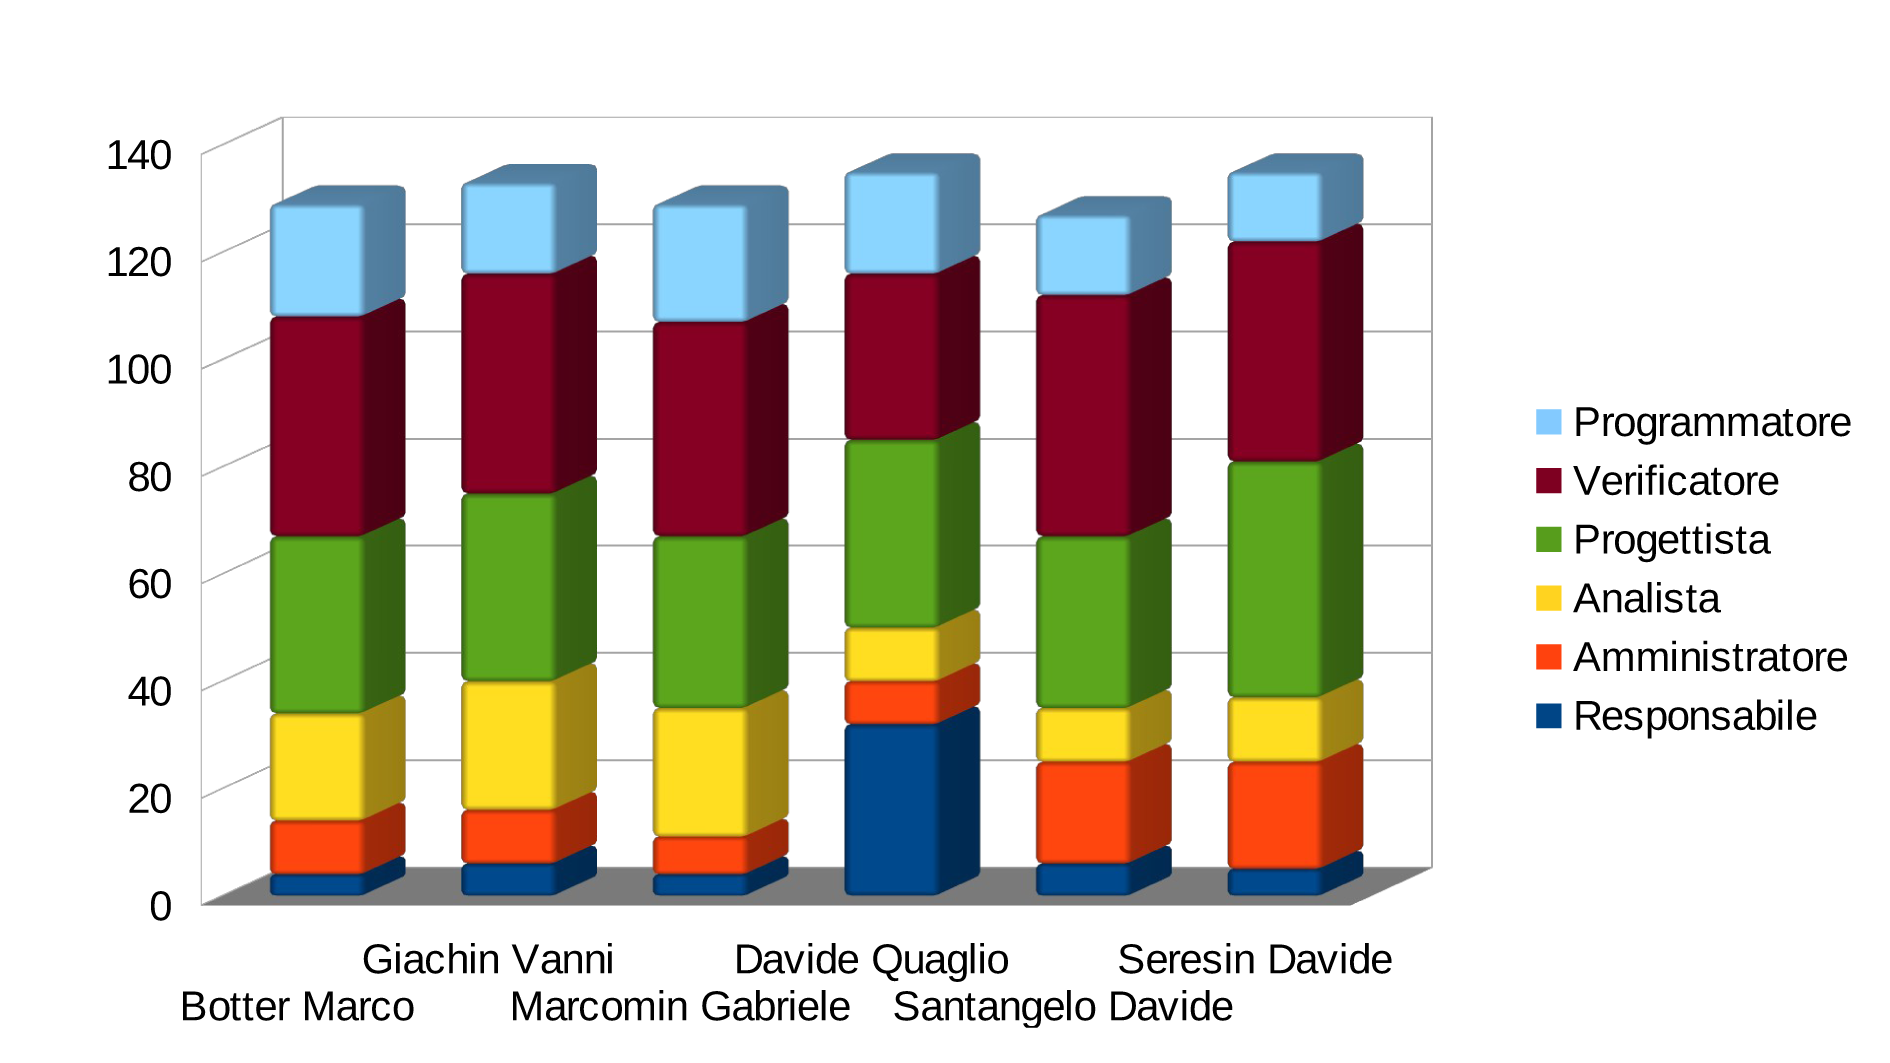
\includegraphics[scale=0.7]{../modello/img/5.png}}
        \end{picture}
\begin{center}
Grafico 5: Grafico ore per componente sul totale.
\end{center}
\subsubsection{Prospetto economico con periodo di Analisi}
\begin{center}
\begin{tabular}{| l | c | c |}
\hline
Ruolo & Ore & Costi \\
\hline
Responsabile & 57 & 1710 \\
Amministratore & 74 & 1480 \\
Analista & 100 & 2500\\
Progettista & 211 & 4642 \\
Verificatore & 237 & 3585 \\
Programmatore & 107 & 1605 \\
\hline
\textbf{Totale} & 788 & 15522 \\
\hline
\end{tabular}
\\
Tabella 11: Tabella del prospetto economico.
\end{center}
\setlength{\unitlength}{1mm}\begin{picture}(15,64)
                \put(10,0){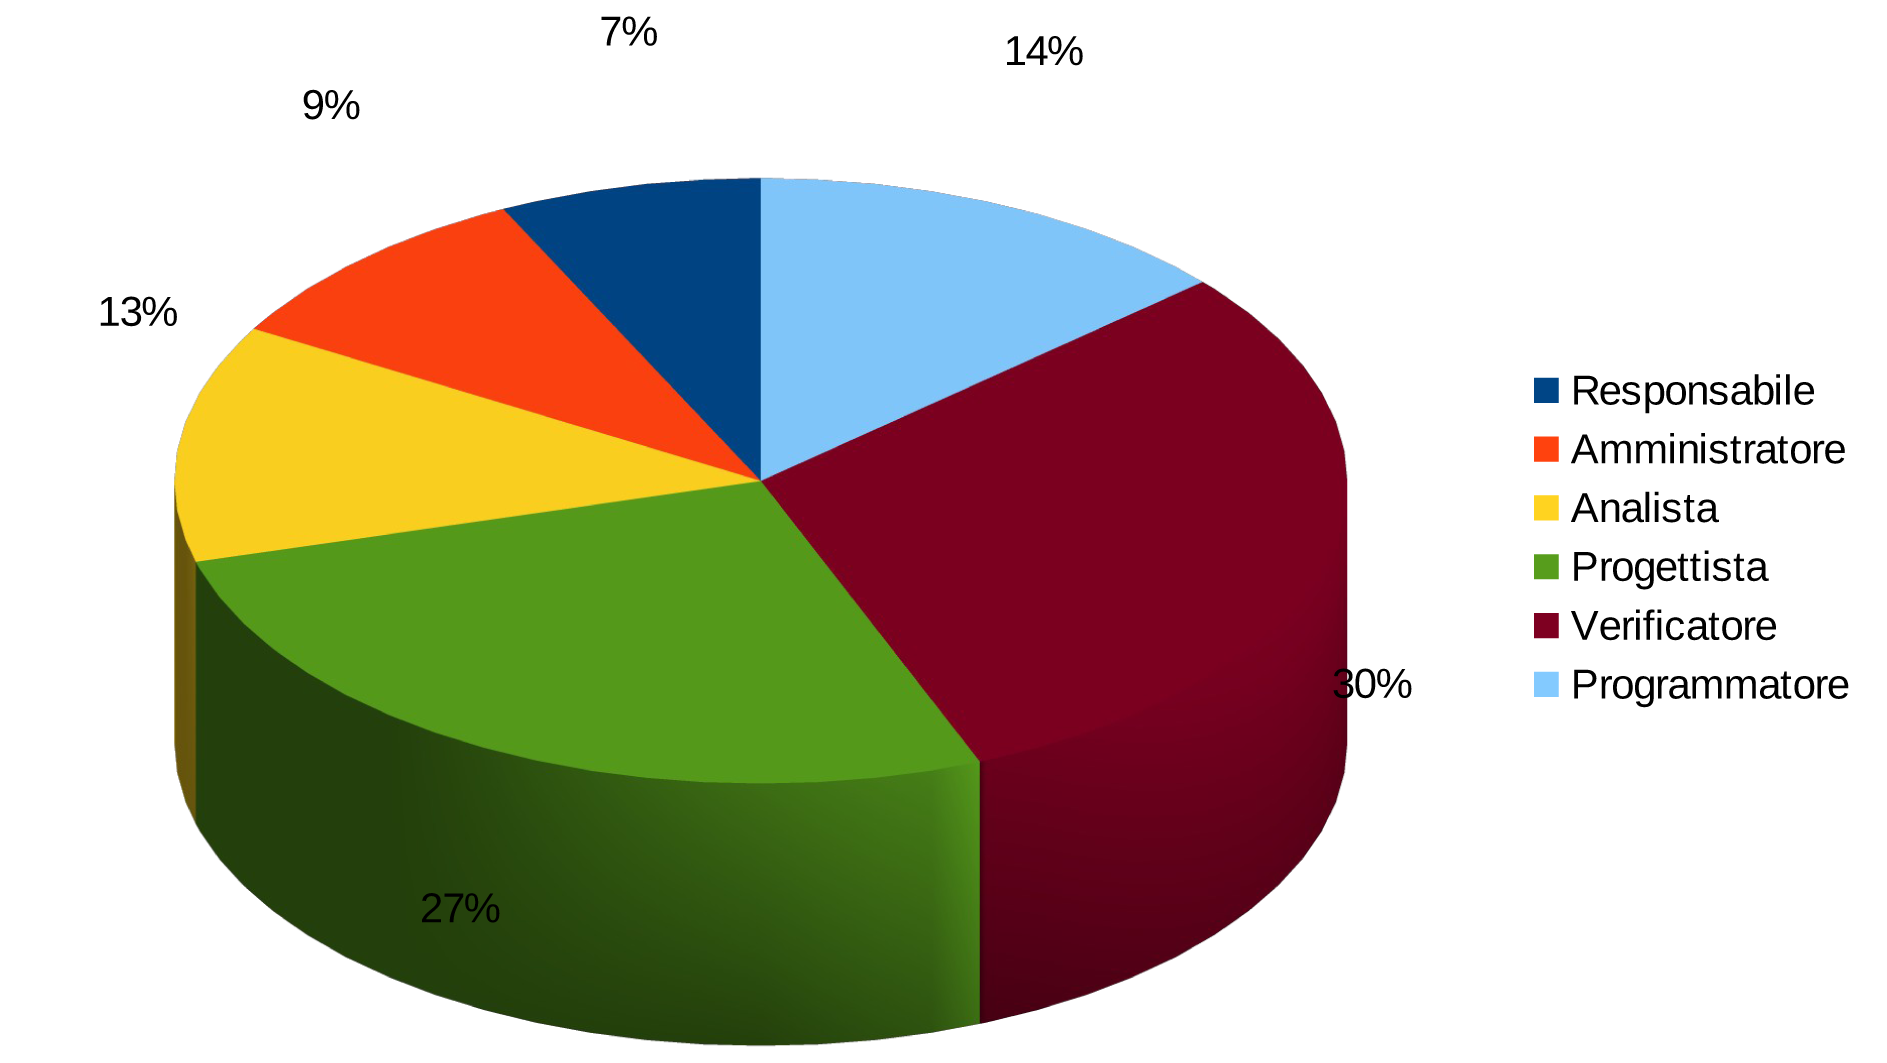
\includegraphics[scale=0.7]{../modello/img/torta5.png}}
    \end{picture}
\begin{center}
Grafico 6: Grafico sulla suddivisione dei compiti.
\end{center}
Si noti come le ore dedicate all'attivit\'a di verifica siano del 30\%.\\
\subsection{Ore rendicontate}
\subsubsection{Prospetto economico}
\begin{center}
\begin{tabular}{| l | c | c |}
\hline
Ruolo & Ore & Costi \\
\hline
Responsabile & 27 & 810 \\
Amministratore & 40 & 800 \\
Analista & 36 & 900\\
Progettista & 211 & 4642 \\
Verificatore & 209 & 3135 \\
Programmatore & 107 & 1605 \\
\hline
\textbf{Totale} & 630 & 11892 \\
\hline
\end{tabular}
\\
Tabella 12: Tabella del prospetto economico senza analisi.
\end{center}
Secondo i risultati ottenuti dalla tabella il costo totale per lo sviluppo del progetto \'e \textbf{11892}\euro~, tuttavia si \'e aggiunto un valore del 10\%, come trattato nella sottosezione \ref{subsubsec:rischiocosti}, poich\'e si \'e tenuta in considerazione l'elevata inesperienza del gruppo e si \'e giunti cos\'i a un totale di \textbf{13081\euro}.